
\subsection{Insegnante}

\subsubsection{Panoramica Insegnante}

\begin{figure}[H]
\centering
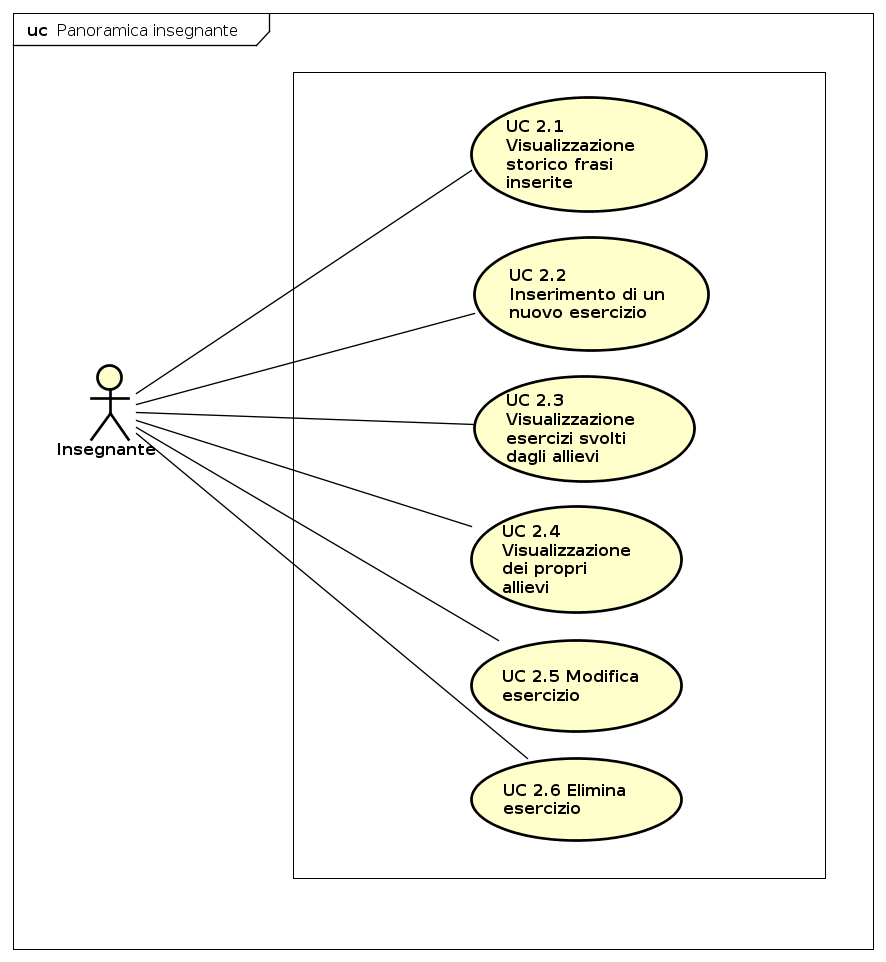
\includegraphics[width=14cm]{img/PanoramicaInsegnanti.png} 
\caption{Panoramica insegnante}
\end{figure}

%MODIFICATO da cambiare uml 
\subsubsection{UC 2.1 Visualizzazione profilo personale}

%\begin{figure}[H]
%\centering
%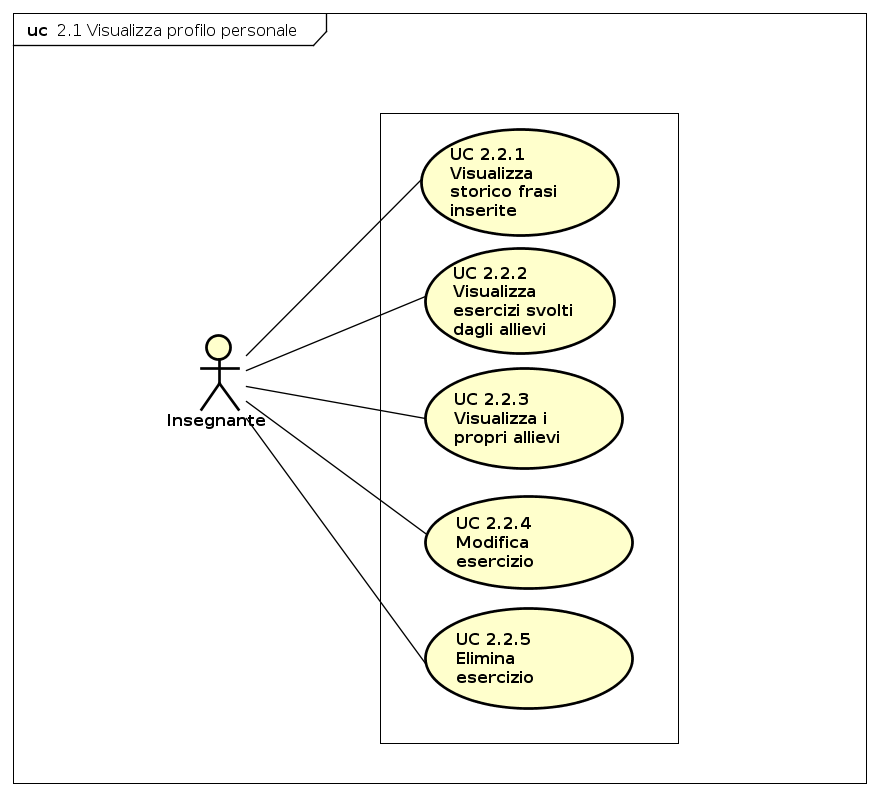
\includegraphics[width=14cm]{img/UC21.png} 
%\caption{Caso d'uso UC 2.1}
%\end{figure}

\begin{itemize}
	\item[•] \textbf{Attori}: Insegnante;
	\item[•] \textbf{Descrizione}: L’insegnante ha accesso al suo profilo personale dove può vedere i suoi dati ed effettuare modifiche agli esercizi;

	\item[•] \textbf{Precondizione}: Il sistema offre l’accesso a una dashboard con tutti i dati;

	\item[•] \textbf{Postcondizione}:  Il profilo personale dell’insegnante è aperto;

\end{itemize}


\subsubsection{UC 2.2 Inserimento di un nuovo esercizio}

\begin{figure}[H]
	\centering
	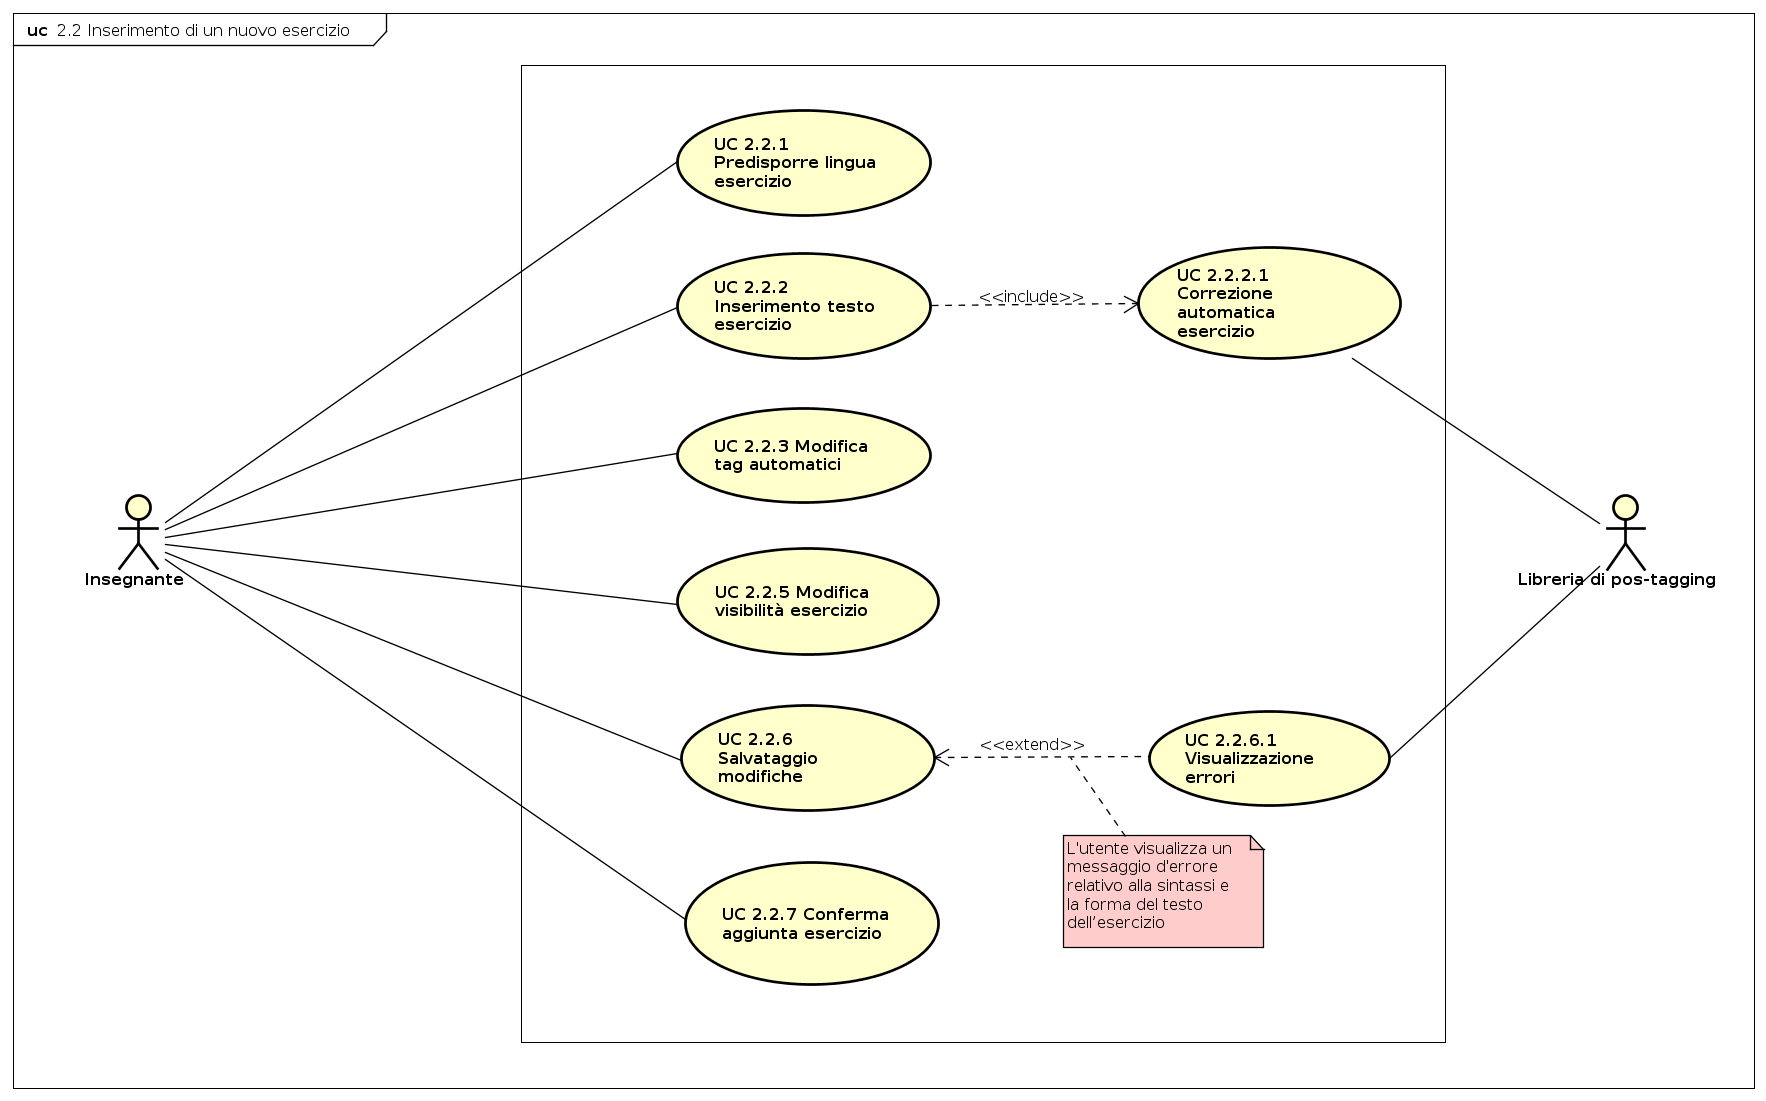
\includegraphics[width=18cm]{img/UC22LIBRERIA.png} 
	\caption{Caso d'uso UC 2.2 interazione con la libreria;}
\end{figure}


\begin{figure}[H]
	\centering
	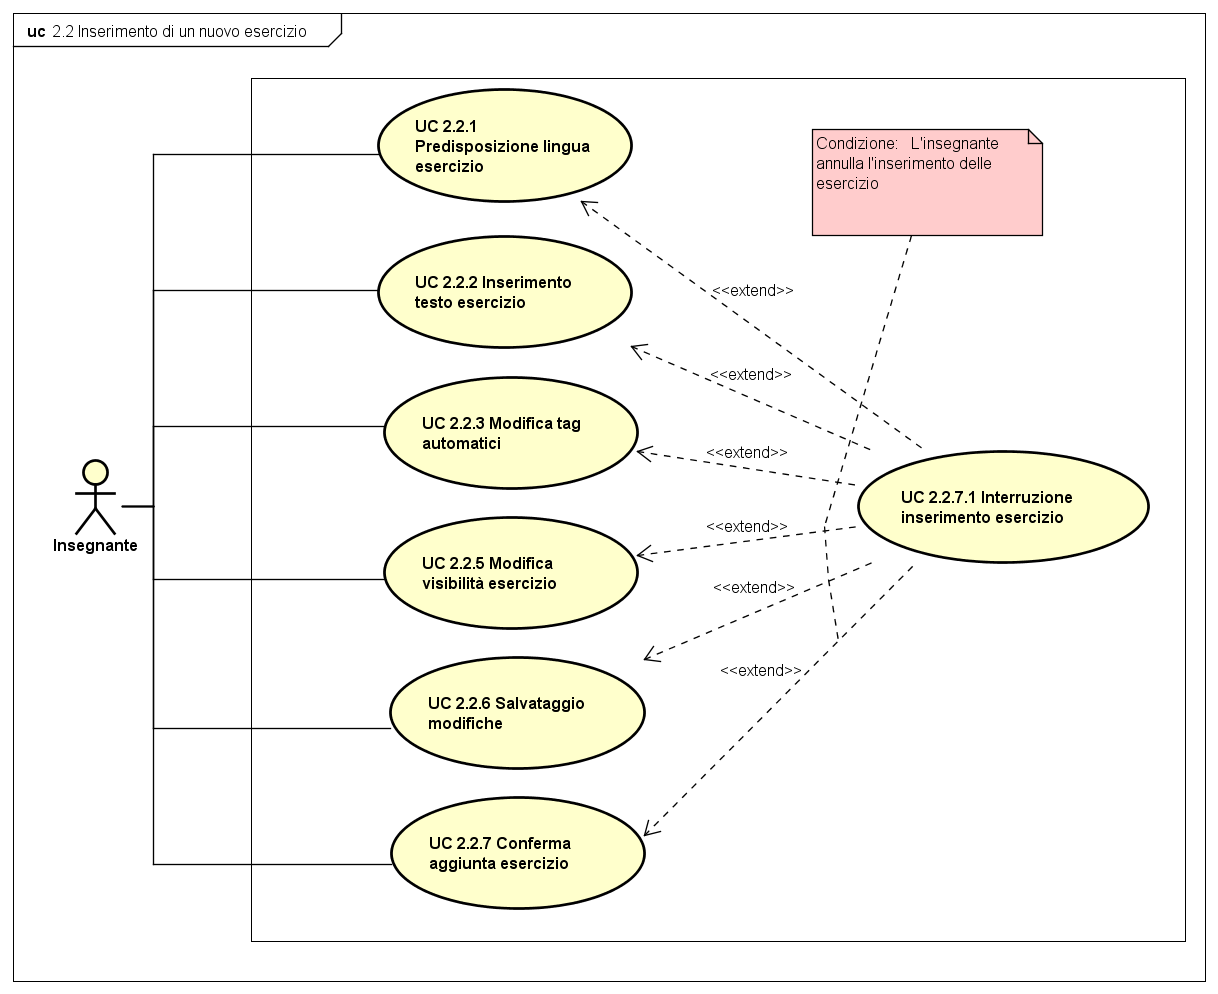
\includegraphics[width=18cm]{img/UC22SISTEMA.png} 
	\caption{Caso d'uso UC 2.2 interazione con il sistema;}
\end{figure}

\begin{itemize}
	\item[•] \textbf{Attori}: Insegnante;
	\item[•] \textbf{Descrizione}: L'insegnante aggiunge attraverso il testo di un nuovo esercizio;
	\item[•] \textbf{Precondizione}: Il sistema offre la possibilità di aggiungere un esercizio nel sistema e l'insegnante non ha aggiunto l'esercizio;
	\item[•] \textbf{Postcondizione}: Un nuovo esercizio è stato aggiunto;
	\item[•] \textbf{Flusso degli eventi}:
	\begin{enumerate}
		\item UC 2.2.1 Predisporre lingua esercizio;
		\item UC 2.2.2 Inserimento testo esercizio;
		\item UC 2.2.3 Modifica tag automatici;

		\item UC 2.2.5 Modifica visibilità esercizio;
		\item UC 2.2.6 Salvataggio modifiche;
		\item UC 2.2.7 Conferma aggiunta esercizio;
	\end{enumerate}
	\item[•] \textbf{Estensioni}:	
	\begin{enumerate}
		\item UC 2.2.6.1 Visualizzazione errori.
		\item UC 2.2.2.1 Correzione automatica esercizio;
		\item UC 2.2.7.1 Interruzione inserimento esercizio.
	\end{enumerate}
	\item[•] \textbf{Flusso degli eventi alternativo}:
	\begin{enumerate}
		\item UC 2.2.4 Inserimento soluzione alternativa;
	\end{enumerate}
\end{itemize}
%mettere altro sub 
\subsubsection{UC 2.2.1 Predisporre lingua esercizio}
\begin{itemize}
	\item[•] \textbf{Attori}: Insegnante;
	\item[•] \textbf{Descrizione}: L'insegnante sceglie la lingua dell’esercizio che vuole scrivere;
	\item[•] \textbf{Precondizione}: Il sistema offre la possibilità di scegliere tra più lingue il testo dell’esercizio;
	\item[•] \textbf{Postcondizione}: La lingua è stata scelta;
\end{itemize}
%mettere altro sub 
\subsubsection{UC 2.2.2 Inserimento testo esercizio}

\begin{itemize}
	\item[•] \textbf{Attori}: Insegnante;
	\item[•] \textbf{Descrizione}: L'insegnante scrive il testo dell’esercizio;
	\item[•] \textbf{Precondizione}: Il sistema offre la possibilità di scrivere un testo;
	\item[•] \textbf{Postcondizione}: Il testo è stato scritto;
\end{itemize}

%mettere altro sub 
\subsubsection{UC 2.2.2.1 Correzione automatica esercizio}
\begin{itemize}
	\item[•] \textbf{Attori}: Insegnante, libreria di {PoS-tagging}\ped{G};
	\item[•] \textbf{Descrizione}: L’insegnante ottiene automaticamente i tag dal testo dell’esercizio attraverso la libreria di PoS-tagging;
	\item[•] \textbf{Precondizione}: L'insegnante ha inserito il testo dell'esercizio;
	\item[•] \textbf{Postcondizione}: Viene visualizzata la soluzione dell'esercizio.
\end{itemize}

%mettere altro sub 
\subsubsection{UC 2.2.3 Modifica tag automatici}
\begin{itemize}
	\item[•] \textbf{Attori}: Insegnante, libreria di PoS-tagging;
	\item[•] \textbf{Descrizione}: L’insegnante modifica i tag generati automaticamente;
	\item[•] \textbf{Precondizione}: Il sistema offre la possibilità di modificare i tag generati con la correzione automatica;
	\item[•] \textbf{Postcondizione}: I tag relativi al testo scritto sono stati modificati.
\end{itemize}
%mettere altro sub 


\subsubsection{UC 2.2.4 Inserimento soluzione alternativa}
\begin{itemize}
	\item[•] \textbf{Attori}: Insegnante;
	\item[•] \textbf{Descrizione}: L'insegnante inserisce tag alternativi all’esercizio;
	\item[•] \textbf{Precondizione}: Il sistema offre la possibilità di inserire più tag per parola ad esercizio;
	\item[•] \textbf{Postcondizione}: Una soluzione alternativa è stata aggiunta.
\end{itemize}

%mettere altro sub 
\subsubsection{UC 2.2.5 Modifica visibilità esercizio}
\begin{itemize}
	\item[•] \textbf{Attori}: Insegnante;
	\item[•] \textbf{Descrizione}: L’insegnante imposta la visibilità dell' esercizio, ovvero quali allievi possono visualizzarlo e sceglierlo;
	\item[•] \textbf{Precondizione}: L'insegnante non ha impostato la visibilità dell'esercizio;
	\item[•] \textbf{Postcondizione}: L’esercizio è stato reso visibile o meno ad un gruppo di utenti.
\end{itemize}
%mettere altro sub 
\subsubsection{UC 2.2.6 Salvataggio modifiche}
\begin{itemize}
	\item[•] \textbf{Attori}: Insegnante;
	\item[•] \textbf{Descrizione}: L'insegnante salva l'esercizio e le possibili modifiche;
	\item[•] \textbf{Precondizione}: Il sistema offre la possibilità di salvare gli esercizi creati;
	\item[•] \textbf{Postcondizione}: L'esercizio è stato salvato.
\end{itemize}
%mettere altro sub 
\subsubsection{UC 2.2.6.1 Visualizzazione errori testo inserito}
\begin{itemize}
	\item[•] \textbf{Attori}: Insegnante;
	\item[•] \textbf{Descrizione}: L'insegnante visualizza gli errori relativi alla sintassi e la forma dell’esercizio che sta creando;
	\item[•] \textbf{Precondizione}: Il sistema offre la possibilità di visualizzare gli errori effettuati nella scrittura del testo;
	\item[•] \textbf{Postcondizione}: L’insegnante visualizza gli errori relativi al testo inserito.
\end{itemize}
%mettere altro sub 

\subsubsection{UC 2.2.7 Conferma aggiunta esercizio}
\begin{itemize}
	\item[•] \textbf{Attori}: Insegnante;
	\item[•] \textbf{Descrizione}: L'insegnante aggiunge un esercizio al sistema;
	\item[•] \textbf{Precondizione}: ’insegnante ha completato la stesura dell'esercizio;
	\item[•] \textbf{Postcondizione}: L’esercizio è stato aggiunto correttamente al sistema.
\end{itemize}





%%%%%%%%%%%%%%%%%%%%
%%%%%% CODICE DA CAMBIARE TUTTI , SI PARTE DA QUI CON UC 2.3 %%%%%%%%%%
%%%%%%%%%%%%%%%%%%%%

\subsubsection{UC 2.3 Visualizzazione storico frasi inserite}

%\begin{figure}[H]
%\centering
%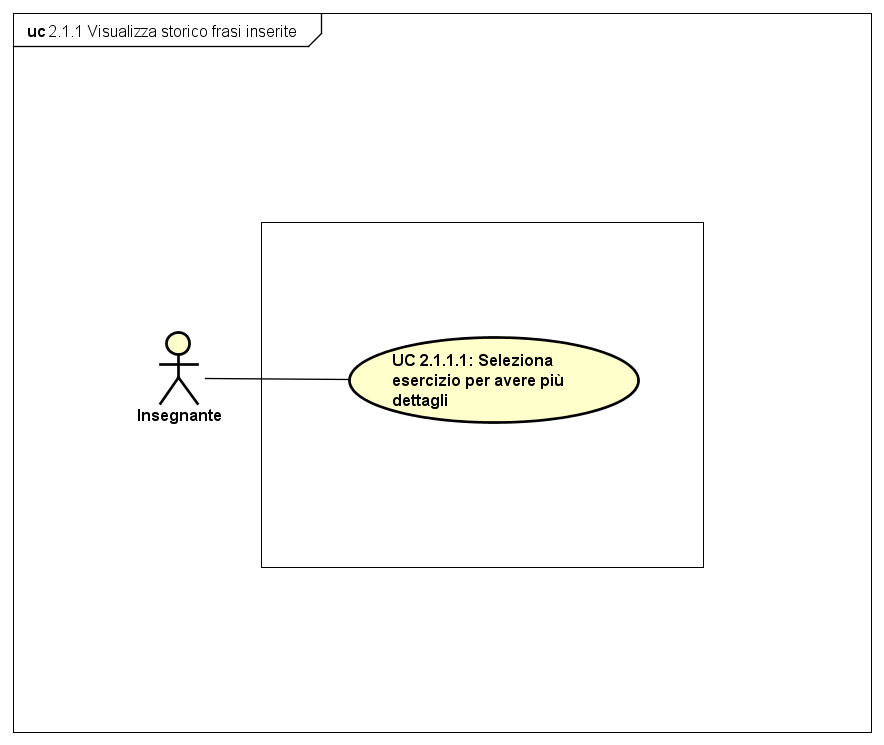
\includegraphics[width=10cm]{img/UC211.png} 
%\caption{Caso d'uso UC 2.1.1}
%\end{figure}

\begin{itemize}
	\item[•] \textbf{Attori}:  Insegnante	   \item[•] \textbf{Descrizione}: L’insegnante visualizza nel suo profilo personale lo storico delle frasi inserite; 
	\item[•] \textbf{Precondizione}: L'insegnante sta visualizzando il proprio profilo personale ;
	\item[•] \textbf{Postcondizione}:  L’insegnante può navigare all’interno della lista di frasi che ha inserito.
\end{itemize}

%mettere altro sub 
\subsubsection{UC 2.3.1 Seleziona esercizio per avere più dettagli}
\begin{itemize}
	\item[•] \textbf{Attori}: Insegnante;
	\item[•] \textbf{Descrizione}:  L’insegnante seleziona dalla lista degli esercizi assegnati un esercizio e ne visualizza i dettagli;
	\item[•] \textbf{Precondizione}: Il sistema offre la possibilità di visualizzare i dettagli relativi ad un esercizio assegnato;
	\item[•] \textbf{Postcondizione}: L’insegnante legge le specifiche dell’esercizio selezionato.
\end{itemize}



%DEVE diventare UC 2.4 DA CAMBIARE TUTTO QUANTO 
\subsubsection{UC 2.4 Visualizzazione esercizi svolti dagli allievi}
%\begin{figure}[H]
%\centering
%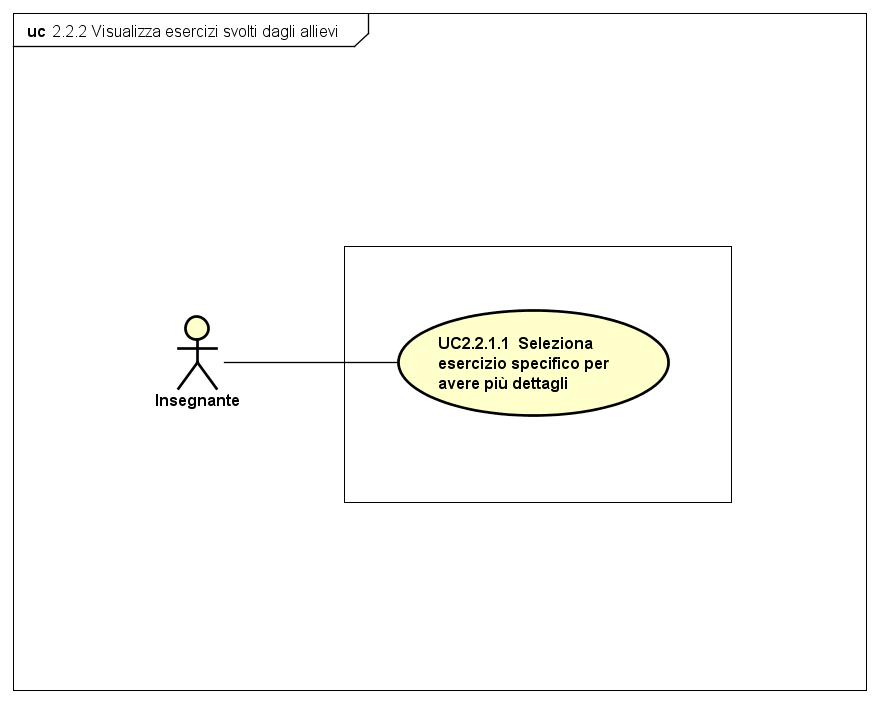
\includegraphics[width=10cm]{img/UC212.png} 
%\caption{Caso d'uso UC 2.1.2}
%\end{figure}
\begin{itemize}
	\item[•] \textbf{Attori}: Insegnante;
	\item[•] \textbf{Descrizione}:  L’insegnante è nella sezione profilo personale e e visualizza l’elenco degli esercizi svolti dagli allievi;
	\item[•] \textbf{Precondizione}:  L’insegnante ha assegnato degli esercizi agli allievi che sono stati svolti;

	\item[•] \textbf{Postcondizione}: L’insegnante visualizza l'elenco degli esercizi svolti svolti dagli allievi; 	
\end{itemize}

\subsubsection{UC 2.5 Visualizzazione dei propri allievi}

%\begin{figure}[H]
%\centering
%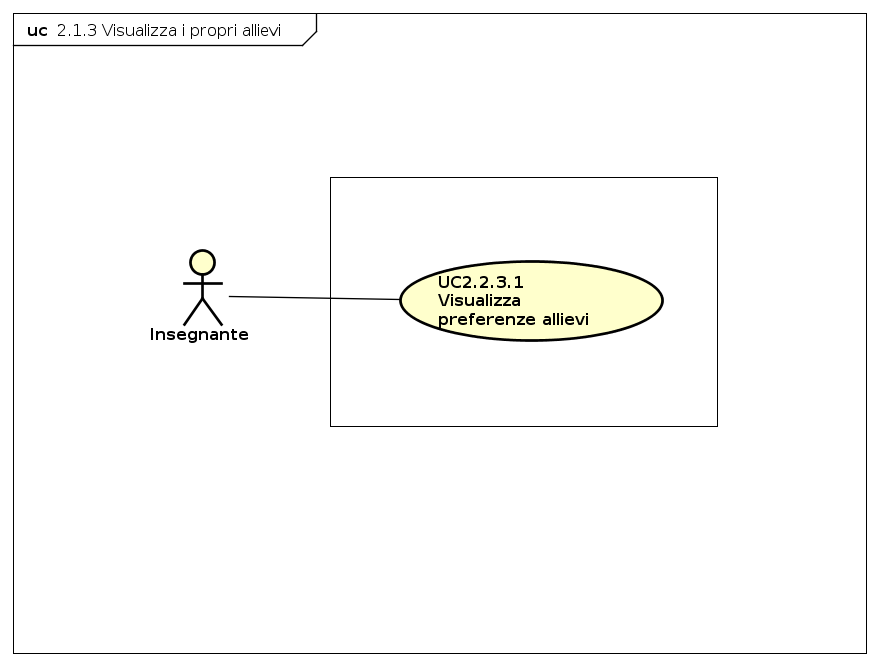
\includegraphics[width=10cm]{img/UC213.png} 
%\caption{Caso d'uso UC 2.1.3}
%\end{figure}

\begin{itemize}
	\item[•] \textbf{Attori}: Insegnante;
	\item[•] \textbf{Descrizione}: L’insegnante visualizza la lista dei suoi allievi;
	\item[•] \textbf{Precondizione}: L'insegnante sta visualizzando il proprio profilo personale;
	\item[•] \textbf{Postcondizione}: L’insegnante visualizza la lista dei propri allievi;
\end{itemize}

%%% da cambiare NUMERO UC va in MODIFICA ESERCIZIO %%%%%%%%%%%%%%


\subsubsection{UC 2.6 Modifica esercizio}
\begin{figure}[H]
\centering
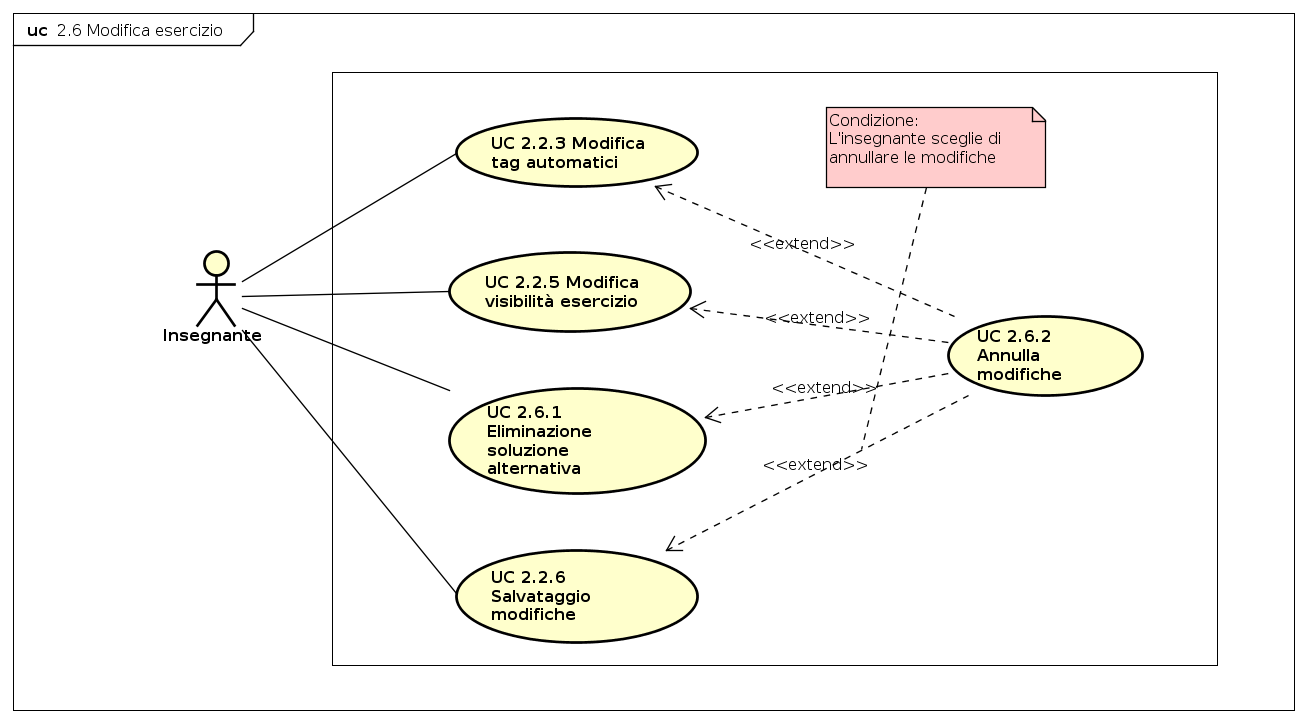
\includegraphics[width=10cm]{img/UC26.png} 
\caption{Caso d'uso UC 2.6}
\end{figure}

\begin{itemize}
	\item[•] \textbf{Attori}: Insegnante;
	\item[•] \textbf{Descrizione}: L’insegnante può modificare un esercizio precedentemente inserito;
	\item[•] \textbf{Precondizione}: Il sistema offre la possibilità di modificare il testo, la
				lingua, la visibilità, i {tag}\ped{G} e le soluzioni alternative 
				dell’esercizio;
	\item[•] \textbf{Postcondizione}: L’esercizio è stato modificato;
	\item[•] \textbf{Flusso degli eventi}:
		\begin{enumerate}
			\item UC 2.2.3 Modifica {tag}\ped{G} automatici;
			\item UC 2.2.5 Modifica visibilità esercizio;
			\item UC 2.6.1 Elimina soluzione alternativa;
			\item UC 2.2.6 Salvataggio modifiche.
		\end{enumerate}
	\item[•] \textbf{Estensioni}
	\begin{enumerate}
		\item UC 2.6.2 Annulla modifiche 
	\end{enumerate}
\end{itemize}   

\subsubsection{UC 2.6.1 Eliminazione soluzione alternativa}
\begin{itemize}
	\item[•] \textbf{Attori}: Insegnante;
	\item[•] \textbf{Descrizione}: L'insegnante elimina una delle soluzioni alternative inserite in precedenza;
	\item[•] \textbf{Precondizione}: Il sistema offre la possibilità di eliminare una soluzione alternativa di un esercizio;
	\item[•] \textbf{Postcondizione}: L'Insegnante ha eliminato una soluzione alternativa di un esercizio.
\end{itemize}

\subsubsection{UC 2.6.2 Annulla modifiche}
\begin{itemize}
	\item[•] \textbf{Attori}: Insegnante;
	\item[•] \textbf{Descrizione}: L'insegnante annulla le modifiche inserite all'interno di un esercizio; 
	\item[•] \textbf{Precondizione}: L'insegnante sta procedendo alla modifica dell'esercizio;
	\item[•] \textbf{Postcondizione}: L'esercizio non è modificato.
\end{itemize}


 
\subsubsection{UC 2.7 Eliminazione esercizio}
\begin{itemize}
	\item[•] \textbf{Attori}: Insegnante;
	\item[•] \textbf{Descrizione}: L'insegnante ha la possibilità di eliminare un esercizio da lei precedentemente inserito;
	\item[•] \textbf{Precondizione}: L'insegnante visualizza nel suo profilo personale lo storico delle frasi inserite;
	\item[•] \textbf{Postcondizione}: L'insegnante ha eliminato l'esercizio precedentemente inserito.
\end{itemize}